El diagrama~\ref{fig:vista-cooperacion-actores} representa a los distintos actores involucrados en el sistema, como estudiantes, administrativos, docentes y el propio grupo de investigación GRID. El diagrama muestra cómo se comunican entre sí y cómo intercambian información, destacando elementos como cursos, programas, relaciones contractuales y archivos. En esencia, este diagrama ilustra las interacciones humanas y organizacionales necesarias para el funcionamiento del sistema.

\begin{figure}[H]
    \centering
    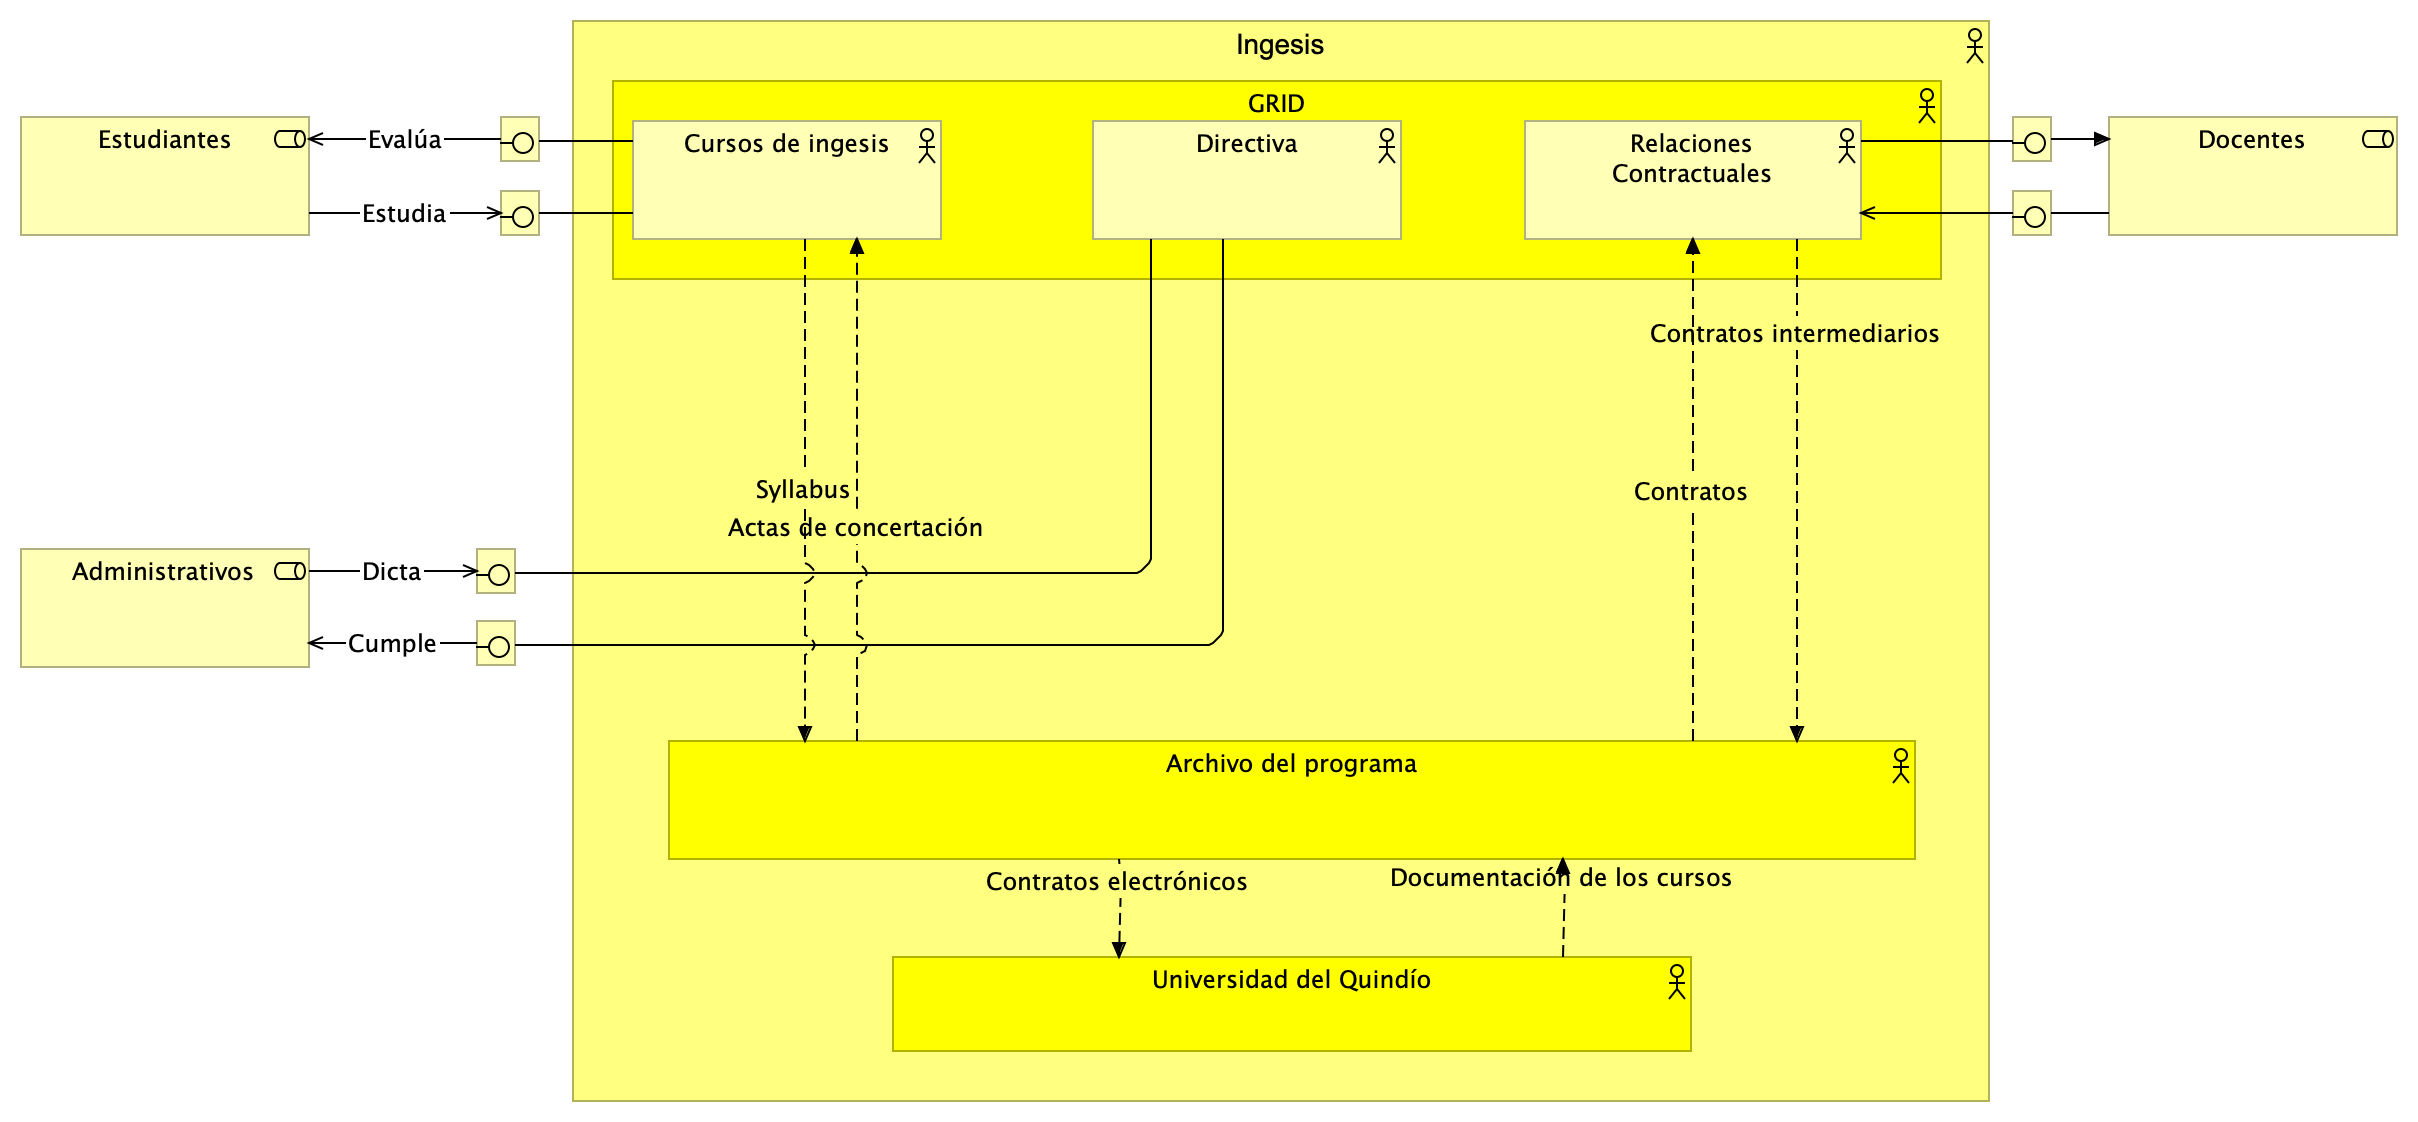
\includegraphics[width=\textwidth]{tablas-images/cp6/Actor-Cooperation-view.png}
    \caption{Vista de Cooperación de Actores}\label{fig:vista-cooperacion-actores}
\end{figure}

La figura~\ref{fig:vista-cooperacion-negocio} describe los procesos que permiten atender solicitudes de recursos tecnológicos, como contenedores, datasets o entornos virtualizados. Se observa cómo el investigador o grupo GRID registra una solicitud, pasa por validaciones, asignación de recursos (CPU, RAM, GPU, almacenamiento) y finalmente se despliega el contenedor. También se contempla la liberación de recursos cuando dejan de usarse. El diagrama integra servicios como autenticación, orquestación de contenedores y repositorios de imágenes, evidenciando cómo se coordinan los distintos procesos de negocio buscando el cumplimiento de objetivos misionales.

\begin{figure}[H]
    \centering
    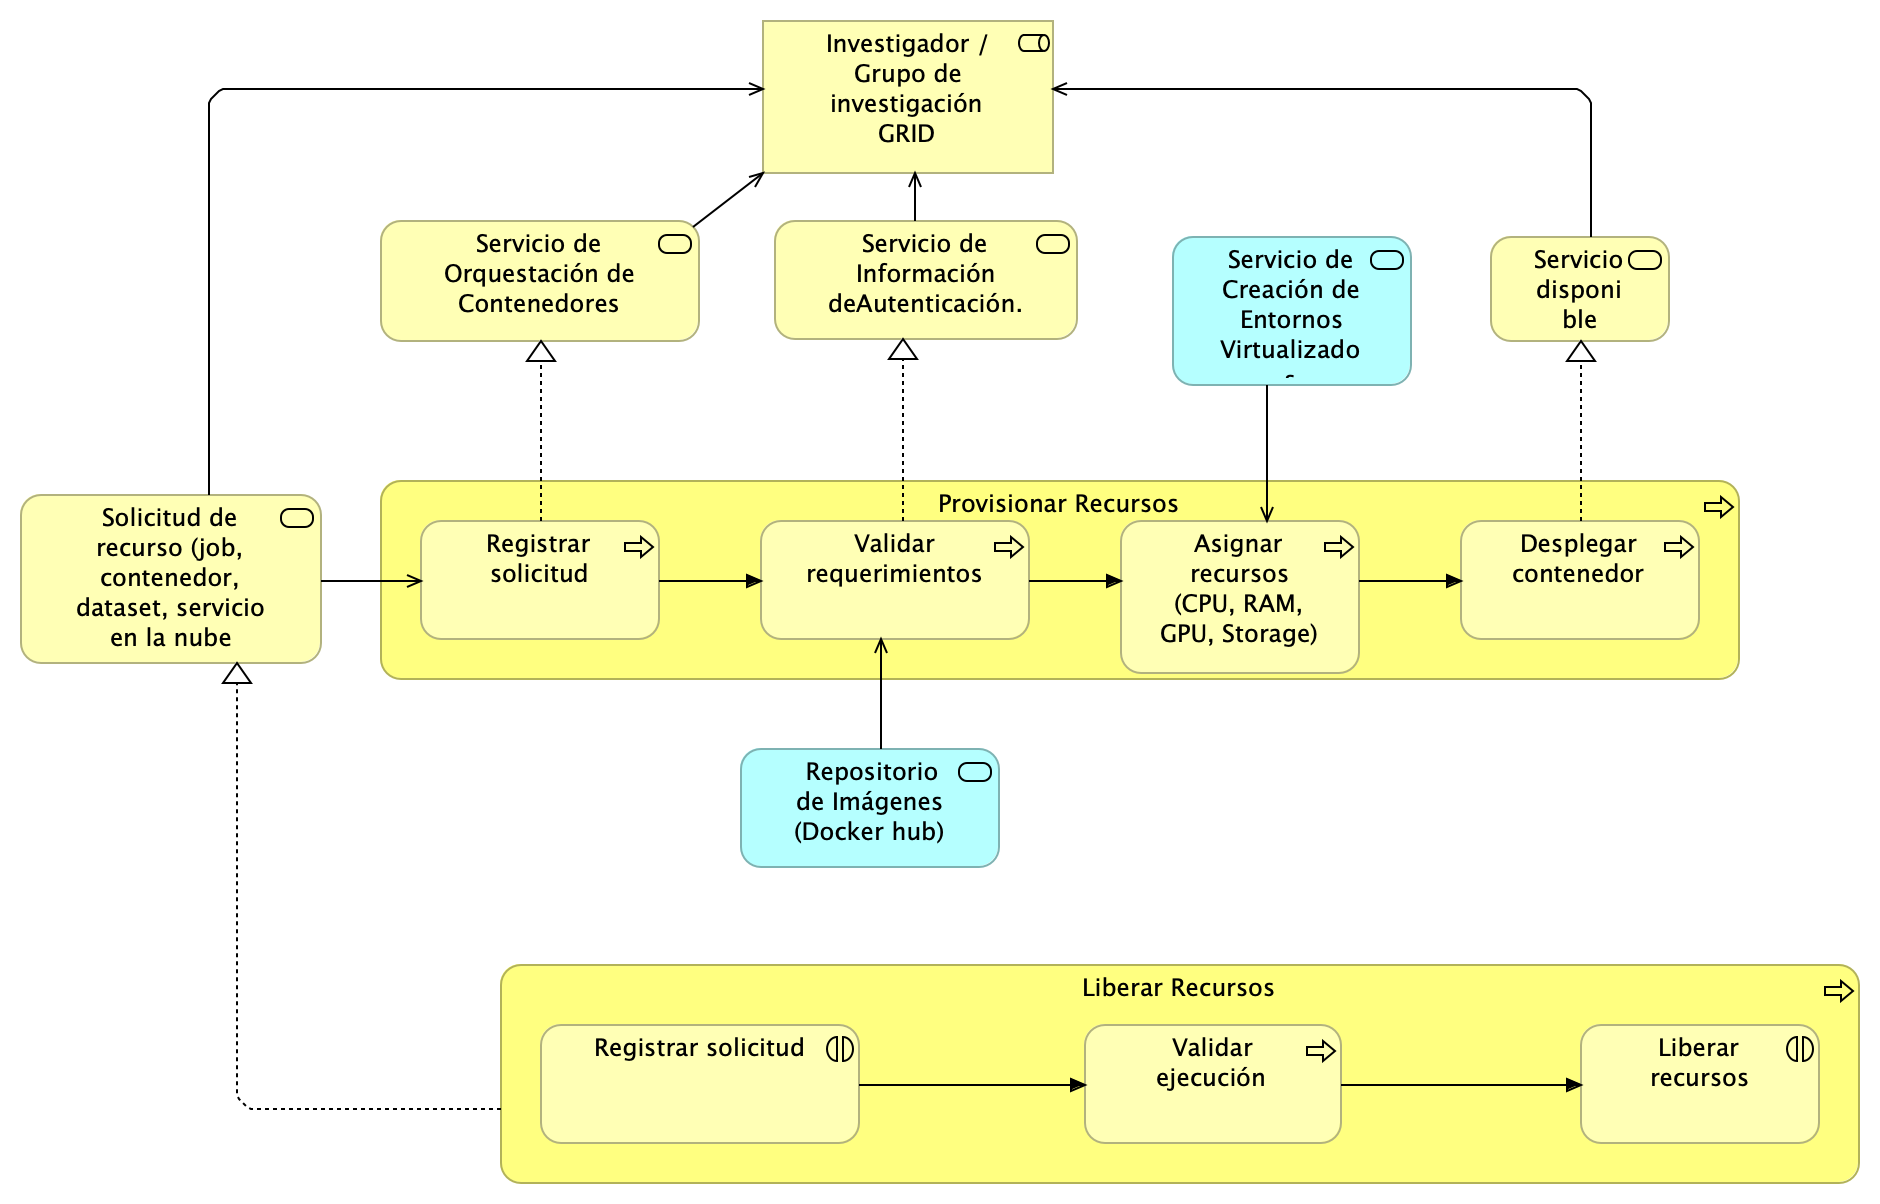
\includegraphics[width=\textwidth]{tablas-images/cp6/Business-Cooperation-View.png}
    \caption{Vista de Cooperación de Negocio}\label{fig:vista-cooperacion-negocio}
\end{figure}

El diagrama~\ref{fig:vista-productos-negocio} ilustra cómo los investigadores y estudiantes acceden a los recursos de cómputo bajo un marco regulado por políticas de uso y respaldado por un SLA. Muestra el flujo desde la solicitud hasta la ejecución de los contenedores, buscando la trazabilidad y control en el consumo de infraestructura.

\begin{figure}[H]
    \centering
    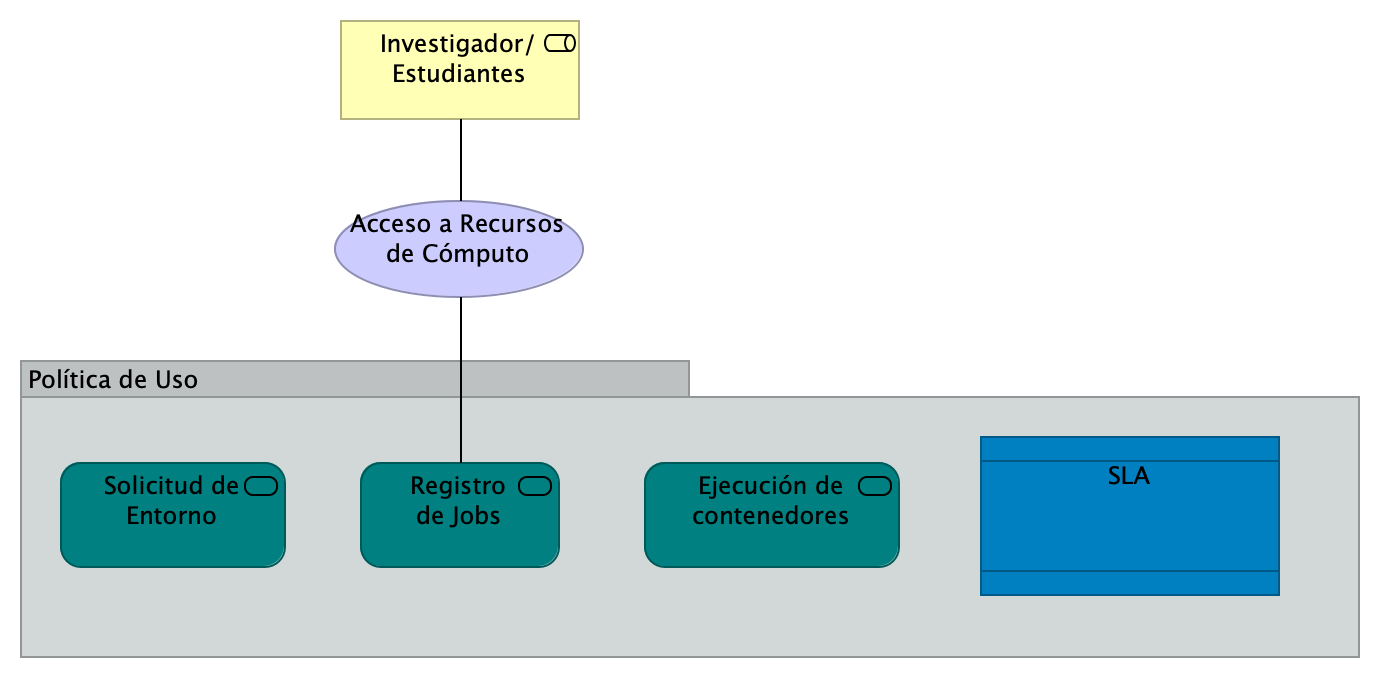
\includegraphics[width=\textwidth]{tablas-images/cp6/Business-Product-View.png}
    \caption{Vista de Producto de Negocio}\label{fig:vista-productos-negocio}
\end{figure}


La imagen~\ref{fig:vista-proceso-negocio} muestra el ciclo de vida completo de los entornos de cómputo: desde la solicitud de ejecución por parte de investigadores o estudiantes, pasando por el registro, validación, planificación de recursos y despliegue, hasta la liberación de los recursos una vez usados. En este flujo intervienen componentes clave como descriptores de jobs en Kubernetes, credenciales de clúster, registros de usuario, acuerdos de recursos, autenticación, orquestador y scheduler de prioridad. En conjunto, el modelo refleja cómo se gestionan de manera controlada y auditable los recursos computacionales dentro del sistema.
\begin{figure}[H]
    \centering
    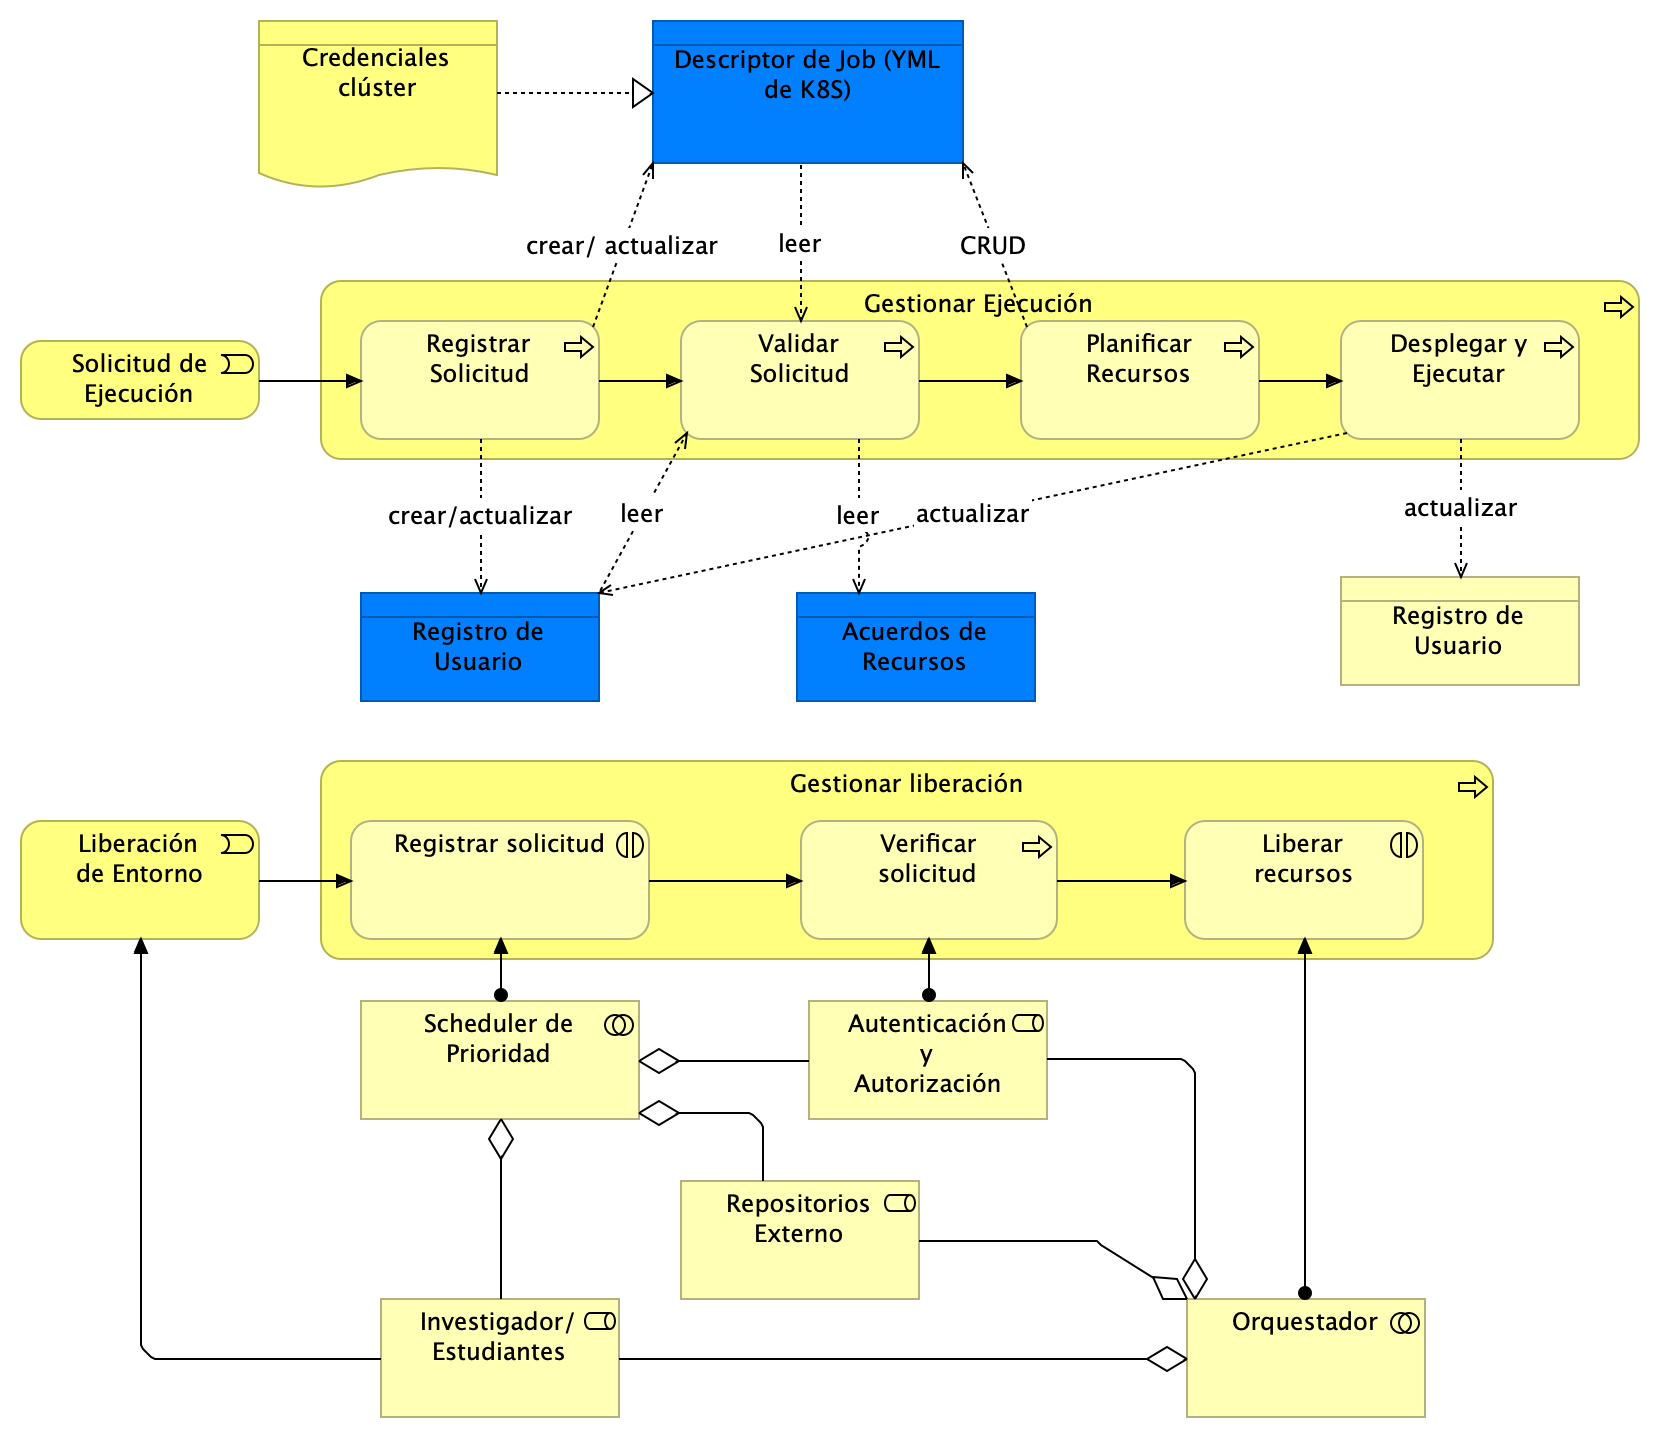
\includegraphics[width=\textwidth]{tablas-images/cp6/Business-Process-View.png}
    \caption{Vista de Proceso de Negocio}\label{fig:vista-proceso-negocio}
\end{figure}

El diagrama ~\ref{fig:vista-funcion-negocio}  muestra cómo la solución de virtualización basada en contenedores del GRID organiza sus principales funciones para dar soporte a estudiantes e investigadores. Entre ellas destacan la gestión de colaboraciones externas, la orquestación de recursos, la gestión de infraestructura virtualizada, la gestión de recursos de cómputo y consumo, la gestión de ejecuciones y la gestión de estudiantes e investigadores. El diagrama refleja la interacción entre actores clave (GRID, estudiantes/investigadores y datacenter Ingesis), señalando el flujo de información, el uso de infraestructura y los resultados de proyectos, lo que permite una administración integral  y alineada con los objetivos académicos y de investigación.

\begin{figure}[H]
    \centering
    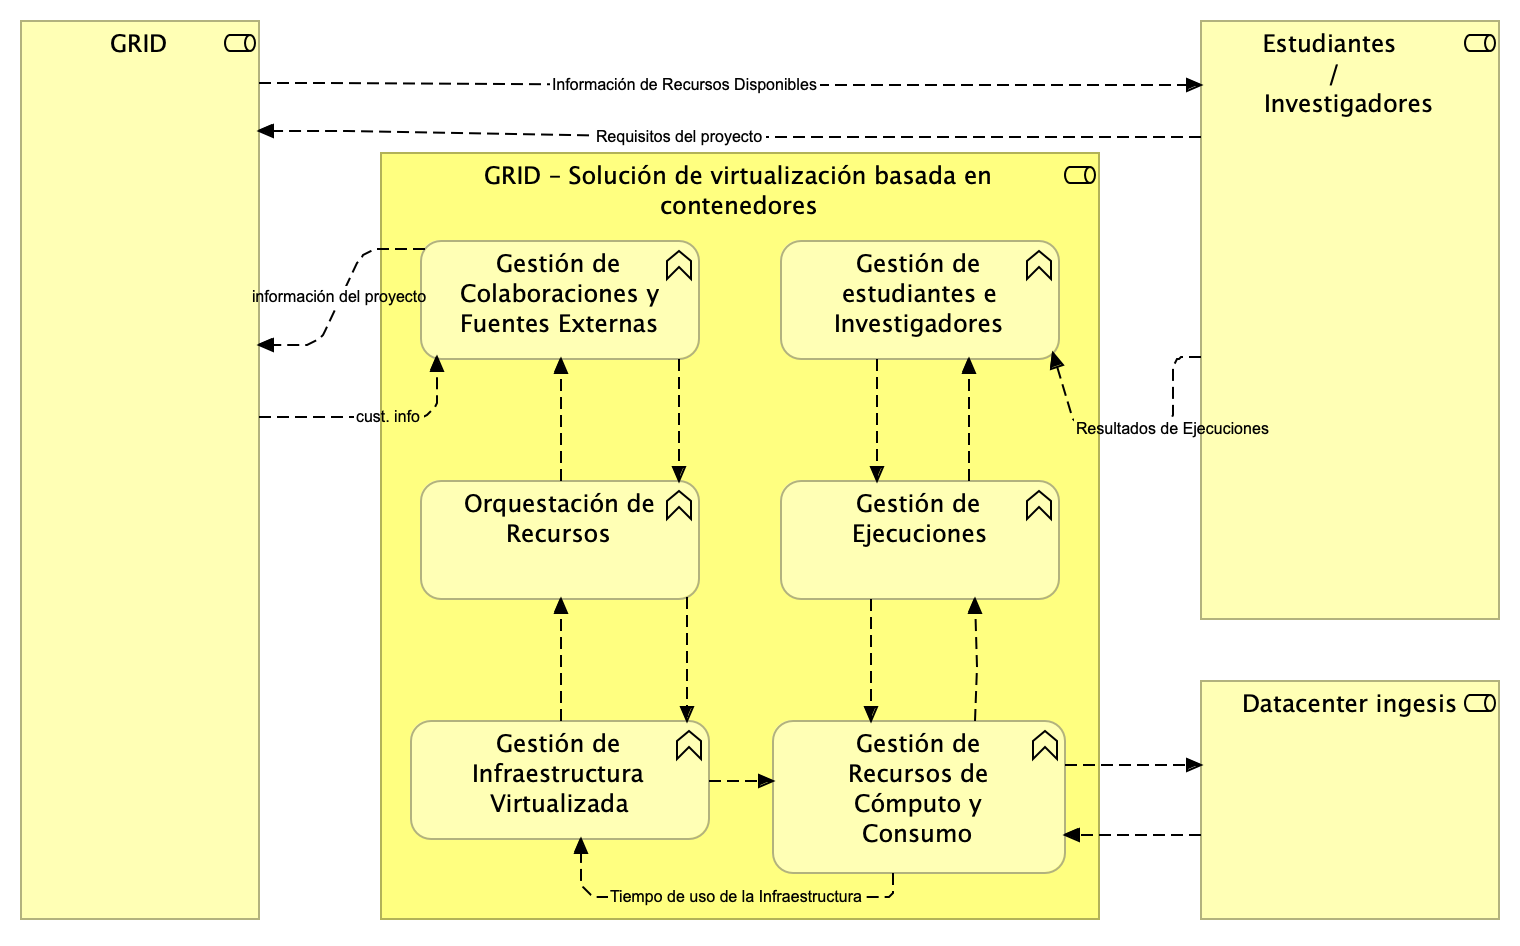
\includegraphics[width=\textwidth]{tablas-images/cp6/Business-Function-View.png}
    \caption{Vista de Función de Negocio}\label{fig:vista-funcion-negocio}
\end{figure}